\documentclass[11pt]{article}
\usepackage{arduino_komp}

\newcommand{\mallurl}{https://wokwi.com/projects/357812594927244289}

% Figures subfolder
\graphicspath{{figures/}}

\begin{document}
\raggedright{}
\begin{center}
  \textbf{\huge{Arduino-kompendium}}
  \huge{-- MEKMEK01}
\end{center}

En samling av teori om hårdvara och tekniker, samt referens för programmering
för att använda Arduino i kursen MEKMEK01 på MTU.

\thispagestyle{empty}
\tableofcontents\label{toc}

\newpage

\section{Teori}
Här förklaras lite grundläggande koncept som behövs för att förstå Arduino.

\subsection{Vad är en pin}\label{sec:pin}
En pin är en fysisk kontakt på en mikrokontroller som kan användas för att
koppla in och ut signaler. En pin kan vara en ingång eller en utgång (se
\ref{sec:io}). De pins som heter D0-D13 kan användas för digitala signaler,
medan A0-A5 kan användas för analoga signaler (se \ref{sec:analog-digital}).

\subsection{Utgång eller ingång?}\label{sec:io}
Du som programmerare väljer om en pin ska vara en ingång eller utgång genom
\texttt{pinMode} (se \ref{sec:pinmode}). En ingång kan användas för att läsa av
en signal, till exempel från en knapp eller en sensor. En utgång kan användas
för att skicka en signal, till exempel till en lampa eller en motor.

\subsection{Digital eller analog?}\label{sec:analog-digital}
En digital signal kan bara ha två tillstånd: hög eller låg. En analog signal
kan ha ett kontinuerligt värde mellan hög och låg. En analog signal kan till
exempel användas för att styra en motor så att den snurrar med olika hastighet,
eller en lampa så att den lyser med olika styrka.

\subsection{PWM}\label{sec:pwm}
Pulse Width Modulation (PWM) är en teknik som används för att skapa en analog
signal
med hjälp av digitala signaler. Detta är användbart för att styra till exempel
motorer och lampor med en mikrokontroller.

PWM fungerar genom att skicka en serie av snabba höga och låga signaler, där
förhållandet mellan hög och låg signal bestämmer hur stark den genomsnittliga
signalen blir.

Se figur \ref{fig:pwm} för att se hur en PWM-signal ser ut vid olika procent.
\begin{figure}[H]
  \centering
  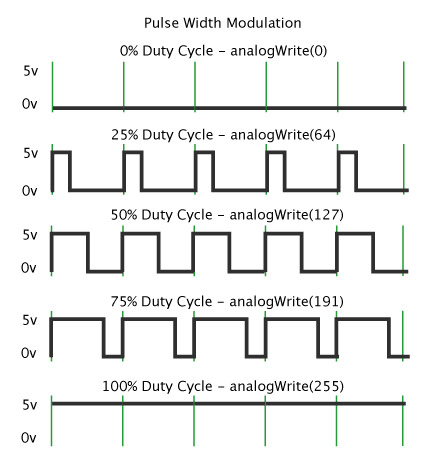
\includegraphics[width=0.5\textwidth]{pwm}
  \caption{Hur PWM-signaler ser ut vid olika procent.}
  \label{fig:pwm}
\end{figure}

\subsection{Enpulsning}\label{sec:enpulsning}
Väldigt ofta är vi intresserade av när en signal precis går från låg till hög
(så kallad \textbf{positiv flank} eller \textbf{rising edge} på engelska), inte
bara \textit{att} signalen är hög. För att detektera en positiv flank kan
enpulsning användas.

Ett sätt att genomföra enpulsning av en signal i Arduino är att spara det förra
tillståndet av signalen, och jämföra det med det nuvarande tillståndet. Om det
förra tillståndet var låg och det nuvarande är högt, har en positiv flank
inträffat.

\textbf{Exempelkod:}
Här enpulsas signalen på pin D2:
\begin{lstlisting}
bool lastState = LOW;
void setup() {
  pinMode(2, INPUT);
}
void loop() {
  bool currentState = digitalRead(2);
  if (lastState == LOW && currentState == HIGH) {
    // En positiv flank har inträffat
  }
  lastState = currentState;
}
\end{lstlisting}

\subsection{Datatyper}
blavlajsadj

\newpage
\section{Programmering}
\subsection{\texttt{pinMode}}\label{sec:pinmode}
Används för att bestämma om en \hyperref[sec:pin]{pin} ska vara en utgång eller
ingång (\ref{sec:io})

\texttt{pinMode} har tre konfigurationer:
\begin{itemize}
  \item \texttt{INPUT}
  \item \texttt{OUTPUT}
  \item \hyperref[sec:input_pullup]{\texttt{INPUT\_PULLUP}}
\end{itemize}

\textbf{Exempelanvändning:}
\begin{lstlisting}
pinMode(4, OUTPUT);
\end{lstlisting}
Kommer att välja pin D4 som en utgång.

\subsubsection{\texttt{INPUT\_PULLUP}}\label{sec:input_pullup}
En variant av \hyperref[sec:input]{input}. Denna konfiguration gör så att
pin:en internt kopplas till en så kallad pull-up resistor.
Det betyder att när pinen inte är kopplad till GND kommer den att vara hög.

Detta är användbart när man kopplar in en knapp, eftersom då behövs endast två
sladdar: en till GND och en till pinen.

\textbf{Obs!} När knappen är nedtryckt kommer alltså signalen vara låg, annars
hög. Det är därför vanligt att man vill invertera den avlästa signalen.

\textbf{Exempelanvändning:}
En knapp kopplad till pin D2:
\begin{lstlisting}
void setup() {
  pinMode(2, INPUT_PULLUP);
}
void loop() {
  bool buttonState = !digitalRead(2); // inverterad logik
  if (buttonState) {
    // Knappen är nedtryckt
  }
}
\end{lstlisting}

\subsection{\texttt{digitalWrite}}
För att styra signaler på en \hyperref[sec:pin]{pin} som är bestämd som
\hyperref[sec:io]{utgång}. Kan användas för att tända eller släcka en lampa,
eller styra en motor. Eftersom en \hyperref[sec:analog-digital]{digital} signal
bara kan vara hög eller låg, kan \texttt{digitalWrite} bara skicka signaler med
dessa två tillstånd.

\textbf{Exempelanvändning:}
För att skicka ut en hög signal på pin D4:
\begin{lstlisting}
digitalWrite(4, HIGH);
\end{lstlisting}

\textbf{Exempelanvändning:}
För att släcka den interna lampan på Arduino-enheten:
\begin{lstlisting}
digitalWrite(LED_BUILTIN, LOW);
\end{lstlisting}

\subsection{\texttt{digitalRead}}
För att läsa av en \hyperref[sec:pin]{pin} som är bestämd som
\hyperref[sec:io]{ingång}. Kan användas för att läsa av en knapptryckning eller
en digital sensor. Returnerar \texttt{HIGH} eller \texttt{LOW} beroende på om
spänningen på pinnen är hög eller låg. Eftersom en
\hyperref[sec:analog-digital]{digital} signal bara kan vara hög eller låg, kan
\texttt{digitalRead} bara läsa av dessa två tillstånd.

Det lämpar sig bra att lagra resultatet i en variabel med typen \texttt{bool}.

\textbf{Exempelanvändning:}
För att läsa av en hög insignal på pin D11:
\begin{lstlisting}
bool value = digitalRead(11);
\end{lstlisting}

\subsection{\texttt{analogWrite}}
För att skriva en \hyperref[sec:analog-digital]{analog} signal till en pin som
är bestämd som \hyperref[sec:io]{utgång}. Den valda pinen måste dessutom vara
en
av de pins som stödjer \hyperref[sec:pwm]{PWM}.

\subsection{\texttt{delay}}
Används för att vänta en viss tid innan programmet fortsätter. Kan användas för
att skapa en paus i programmet, till exempel för att blinka en lampa med ett
visst intervall.

\textbf{Exempelanvändning:}
För att tända en lampa på pin D4 i 1000 millisekunder, sedan släcka den i 1000
millisekunder:

\begin{lstlisting}
digitalWrite(4, HIGH);
delay(1000);
digitalWrite(4, LOW);
delay(1000);
\end{lstlisting}

\textbf{En varning:} många problem kan uppstå om \texttt{delay} används i
större
program, eftersom programmet inte kan göra något annat under tiden som
\texttt{delay} körs. Det finns bättre sätt att vänta i programmet, till exempel
\hyperref[sec:millis]{\texttt{millis}}.

\subsection{Seriell kommunikation}
\subsubsection{\texttt{Serial.begin}}
Måste alltid anropas i \texttt{void setup()} för att överhuvudtaget kunna
använda seriell kommunikation. Argumentet är den baudrate som ska användas. En
standard-baudrate är 9600.

\textbf{Exempelanvändning:}
För att starta seriell kommunikation med baudrate 9600:
\begin{lstlisting}
Serial.begin(9600);
\end{lstlisting}

\subsubsection{\texttt{Serial.print}}\label{sec:serial.print}
Används för att skicka meddelanden genom seriell kommunikation. Vanligtvis vill
man också att en radbrytning ska skickas efter meddelandet, vilket kan göras
med \hyperref[sec:serial.println]{\texttt{Serial.println}.}

\textbf{Exempelanvändning:}
För att skicka texten ``Hello, world!'' till seriell kommunikation:
\begin{lstlisting}
Serial.print("Hello, world!");
\end{lstlisting}

\subsubsection{\texttt{Serial.println}} \label{sec:serial.println}
Har exakt samma användning som
\hyperref[sec:serial.print]{\texttt{Serial.print}} med skillnaden att den
skickar en radbrytning efter meddelandet. Om man vill använda den seriella
plottern är det enklast att använda \texttt{Serial.println}.

\textbf{Exempelanvändning:}
För att skriva ut antalet millisekunder sedan Arduino-enheten startades varje
loop:

\begin{lstlisting}
void loop() {
  Serial.println(millis());
}
\end{lstlisting}

\subsection{\texttt{millis}}\label{sec:millis}
Används för att mäta tid. Vid anrop returneras antal millisekunder sedan
Arduino-enheten startades. En begränsning är att det inte går att mäta längre
tid än vad datatypen \texttt{unsigned long} kan rymma, vilket är ungefär 50
dagar.

\textbf{Exempelanvändning:}\\
För att blinka en lampa varje sekund, utan att använda \texttt{delay}:
\begin{lstlisting}
void loop() {
  unsigned long currentTime = millis(); // Hämta aktuell tid i millisekunder
  // Kontrollera om tillräcklig tid har passerat sedan senaste blinkningen
  if (currentTime - lastTime >= interval) {
    digitalWrite(ledPin, !digitalRead(ledPin)); // Byt tillstånd på lampan
    lastTime = currentTime; // Uppdatera senaste tiden
  }
}
\end{lstlisting}

\end{document}